\begin{figure}
\begin{fullwidth}
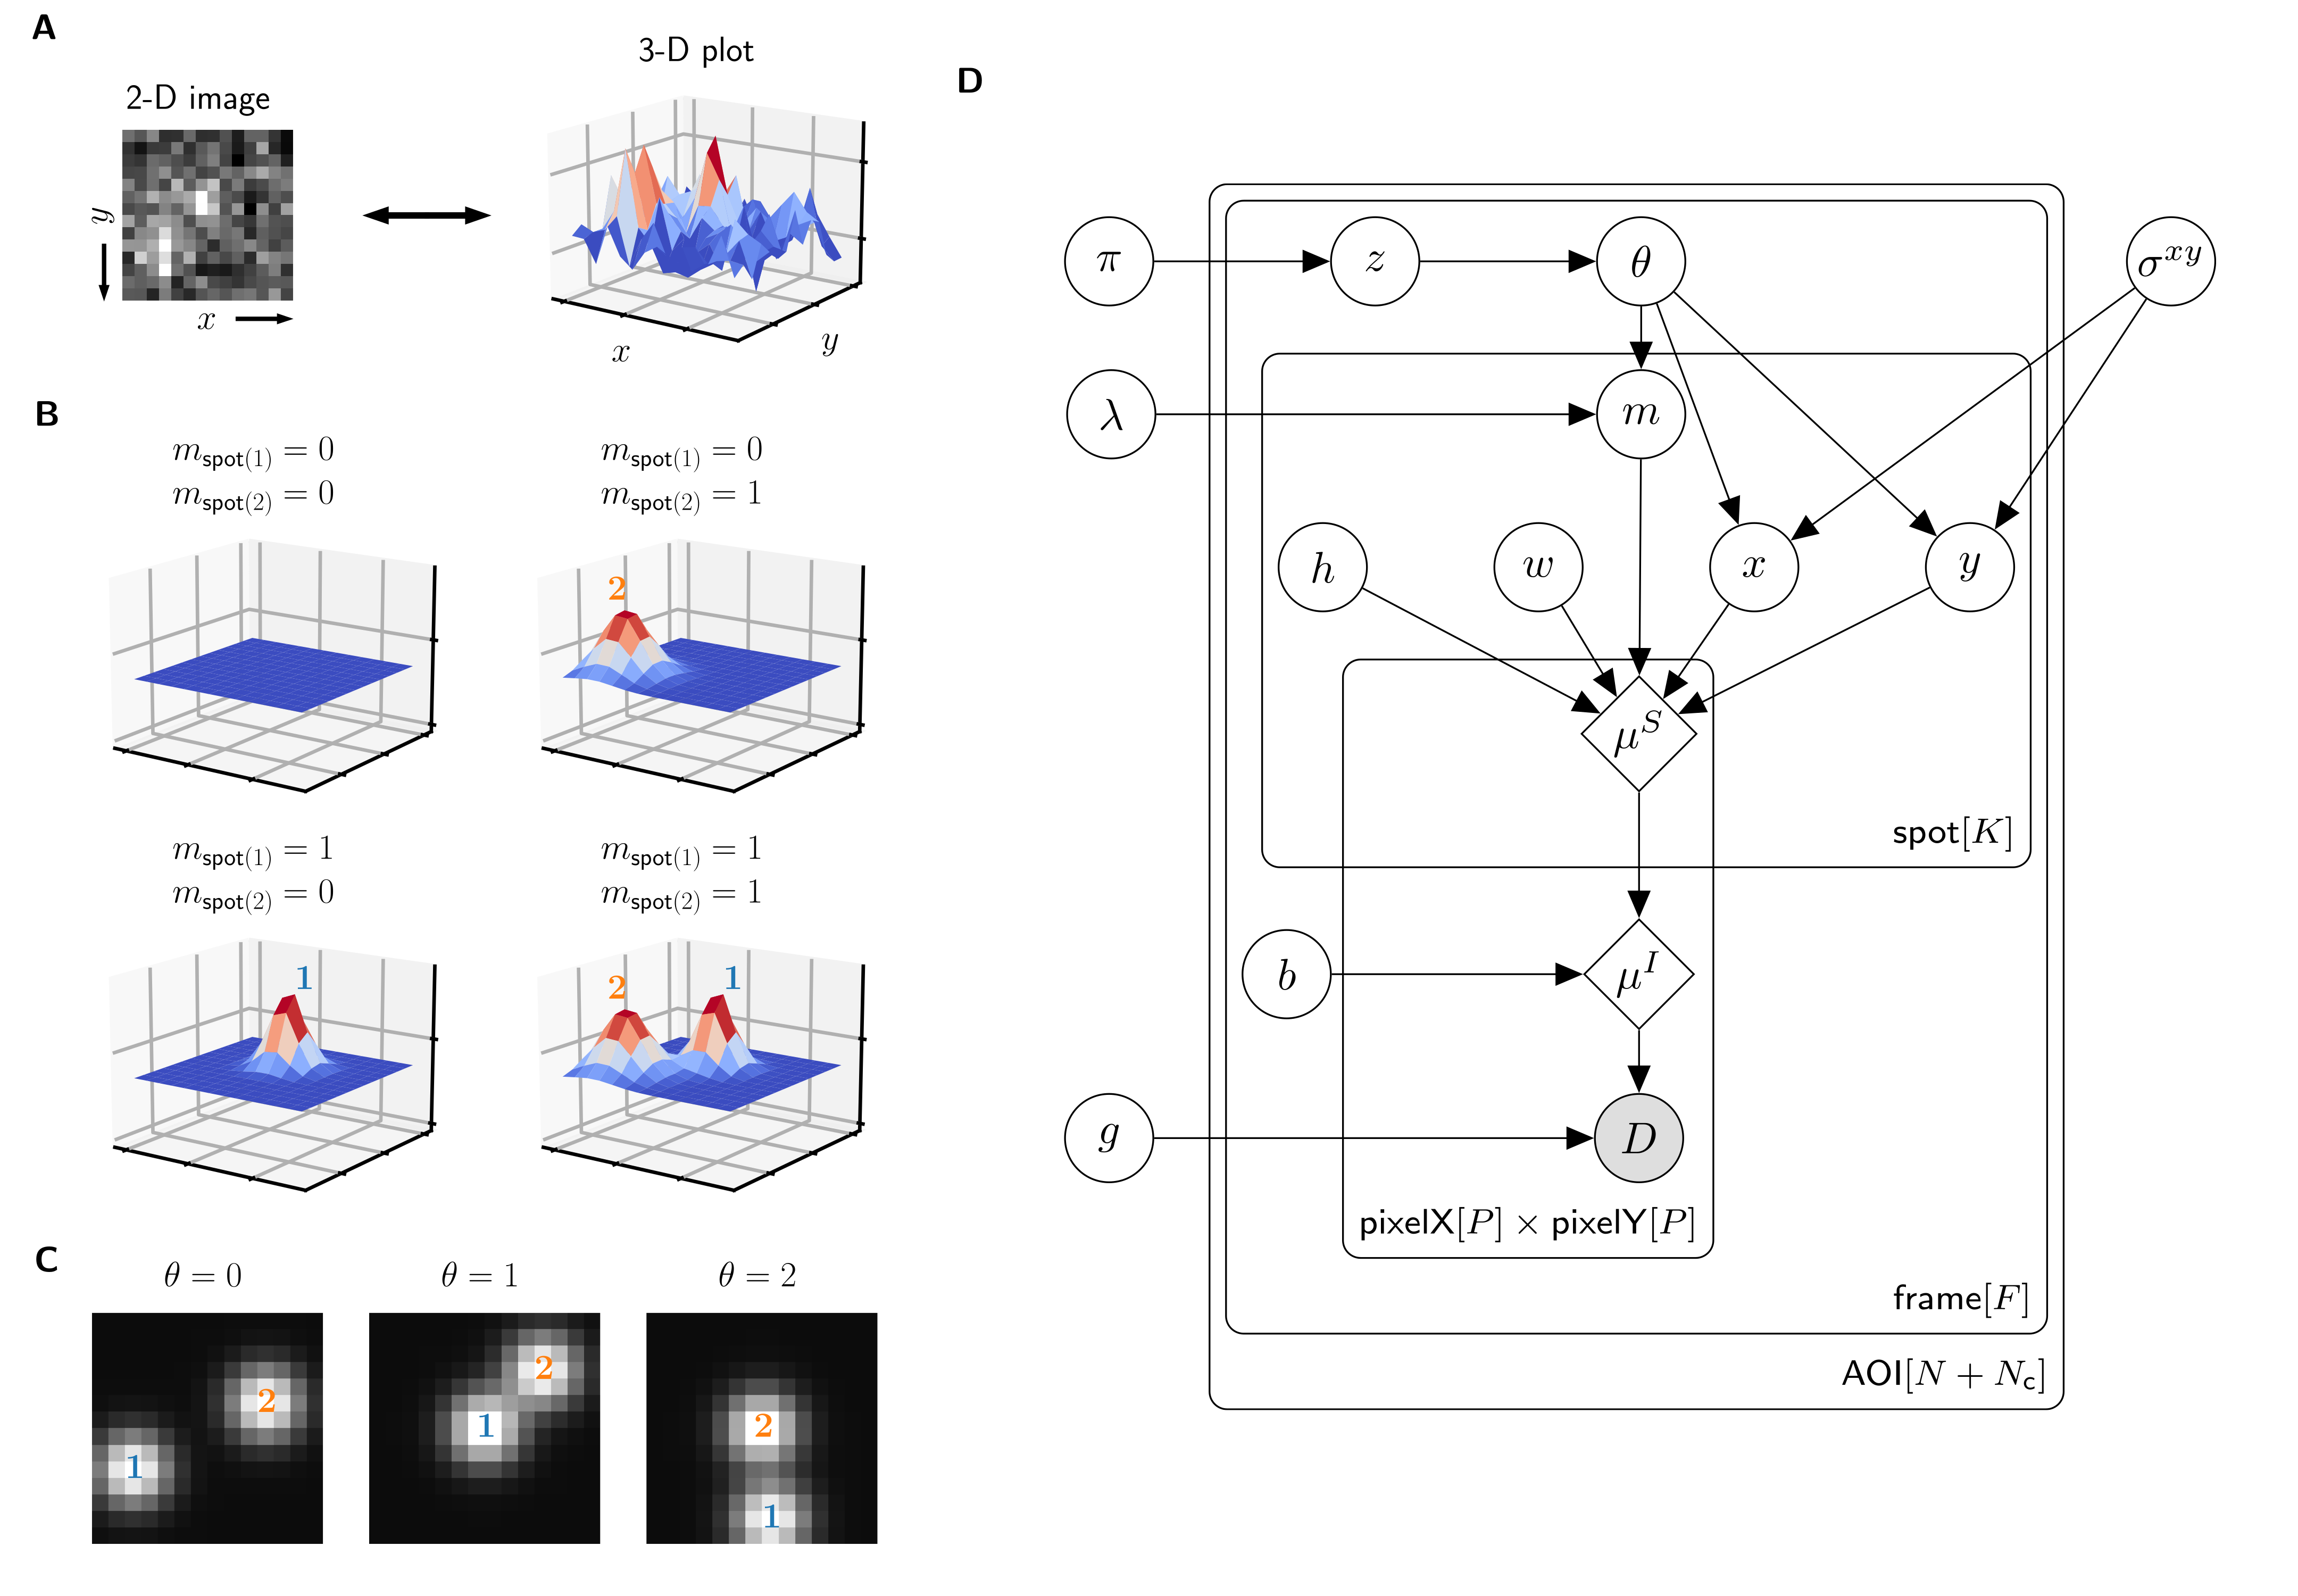
\includegraphics[width=183mm]{figures/graphical_model.png}
\caption{\textbf{Depiction of the probabilistic image model and model parameters.} (\textbf{A}) Example AOI image from the Data set A in \TABLE{datasets}. The AOI image is a matrix of $14 \times 14$ pixel intensities which is shown here as both a 2-D grayscale image and as a 3-D intensity plot. The image contains two spots, one is centered at target location (image center) and the other is located off-target. (\textbf{B}) Examples of four idealized noise-free image representations ($\mu^I$). Image representations consist of zero, one, or two idealized spots ($\mu^S$) superimposed on a constant background ($b$). Each fluorescent spot is represented as a 2-D Gaussian parameterized by integrated intensity ($h$), width ($w$), and position ($x$, $y$). The presence of spots is encoded in the binary spot existence indicator $m$. (\textbf{C}) Simulated idealized images illustrating different values of the target-specific spot index parameter $\theta$. $\theta = 0$ corresponds to a case when no specifically bound molecule is present; $\theta = 1$ or 2 corresponds to the cases in which the specifically bound molecule is spot 1 or 2, respectively. (\textbf{D}) Condensed graphical representation of the probabilistic model. Model parameters are depicted as circles and deterministic functions as diamonds. Observed image ($D$) is represented by a shaded circle. Related nodes are connected by edges, with an arrow pointing towards the dependent node (e.g., the shape of each 2-D Gaussian spot $\mu^S$ depends on spot parameters $m$, $h$, $w$, $x$, and $y$). Plates (rounded rectangles) contain entities that are repeated for the number of instances displayed at the bottom-right corner: number of total AOIs ($N+N_\mathsf{c}$), frame count ($F$), and maximum number of spots in a single image ($K=2$). Parameters outside of the plates are global quantities that apply to all frames of all AOIs. A more complete version of the graphical model specifying the relevant probability distributions is given in \FIGSUPP[graphical_model]{extended}a. }
\label{fig:graphical_model}
\figsupp[Extended graphical representation of the generative probabilistic model and the prior distributions for $x$ and $y$ spot position parameters.]{\textbf{Extended graphical representation of the generative probabilistic model and the prior distributions for $x$ and $y$ spot position parameters.} \textbf{a}, Directed factor graph representation \cite{Bishop2006-oa} of model parameters and parameter distributions. This diagram is a more complete version of the graphical model shown in \FIG{graphical_model}d; it includes additional parameters ($\mu^b$, $\sigma^b$, $\delta$) and explicitly specifies the relevant probability distributions.  Model parameters are depicted as circles, parameter distributions as small filled squares, and deterministic functions as diamonds. Names of the probability distributions are written next to the squares. Input parameters and output parameters are connected by lines, with an arrow pointing towards the dependent parameter. Observed image ($D$) is the sum of the noisy photon-dependent image ($I$) and the photon-independent camera offset ($\delta$). Plates (rounded rectangles) contain nodes that are repeated for the number of instances displayed at the bottom-right corner: number of AOIs ($N+N_\mathsf{c}$), frame count ($F$), maximum number of spots in a single image ($K$), and number of image pixels ($P \times P$). \textbf{b}, Prior distributions of $x$ and $y$ for specific and non-specific binding. Probability densities for $x$ and $y$ are defined in the range $\left[ -(P+1)/2, (P+1)/2 \right] $ relative to the target molecule and are conditional on the identity of the spot (specific or non-specific).  Probability densities for $x$ and $y$ parameters are identical. }{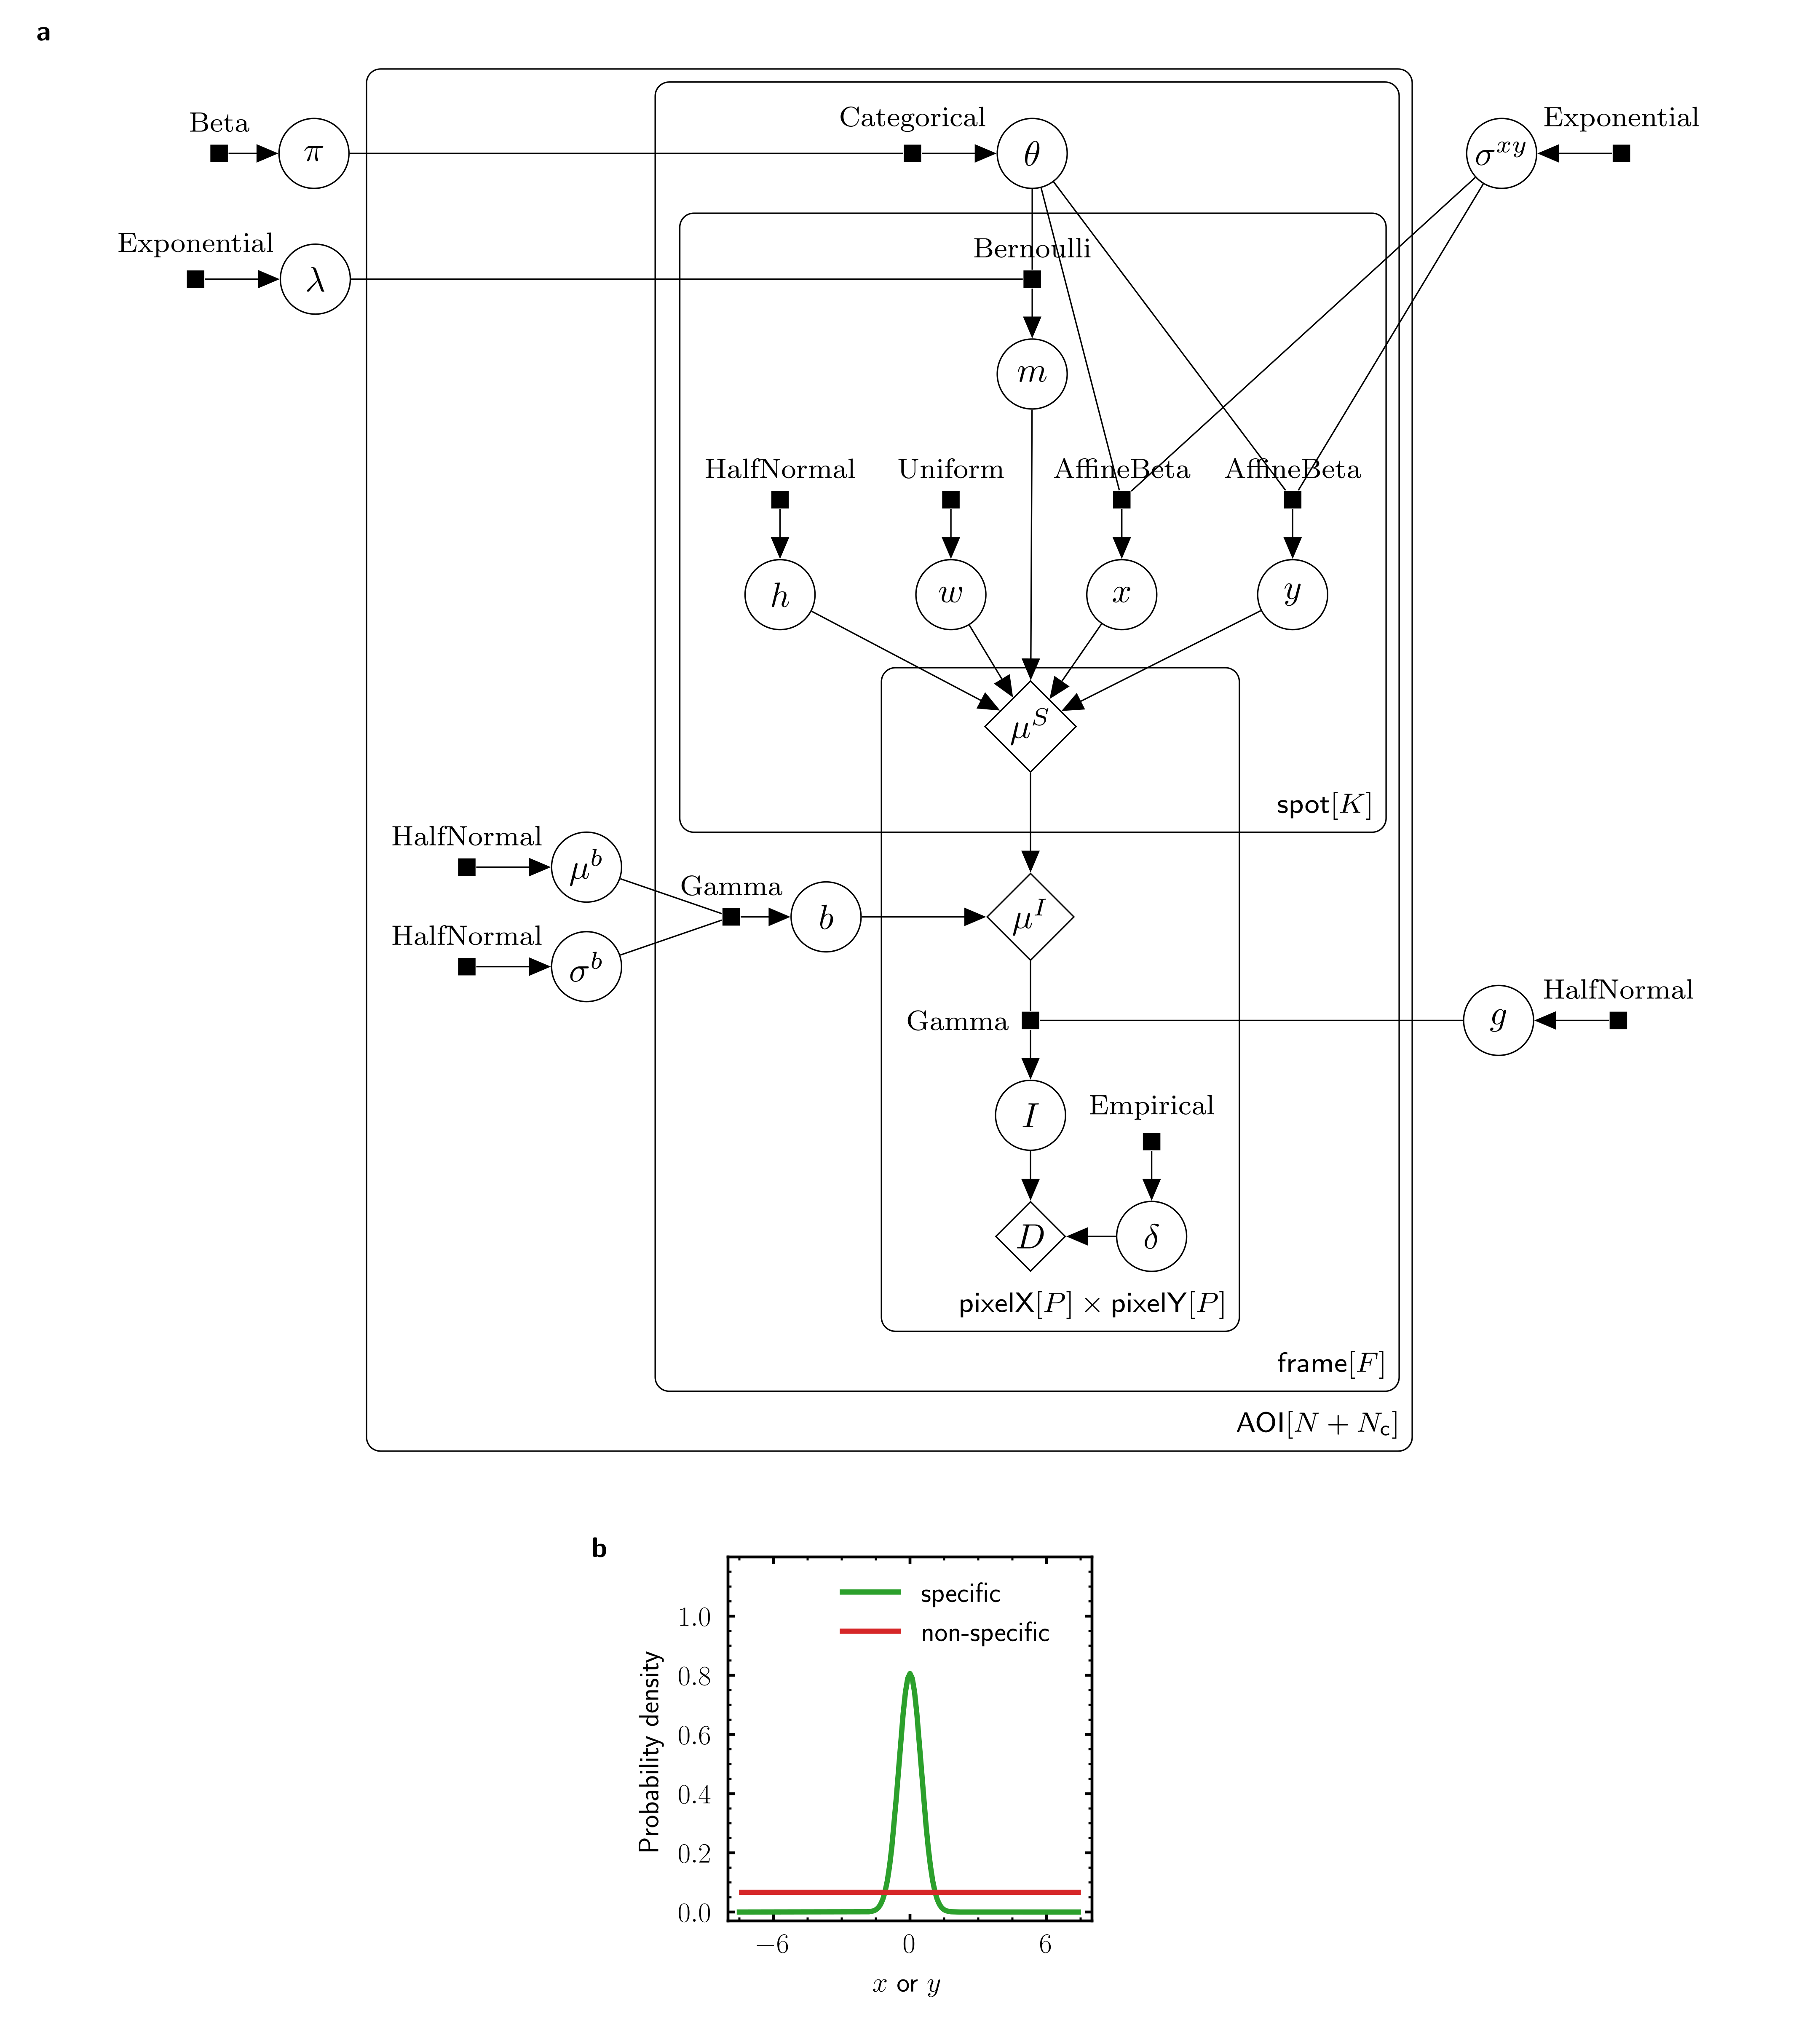
\includegraphics[width=183mm]{extended-data/figure1.png}}\label{figsupp:extended}
\end{fullwidth}
\end{figure}